%!TeX root = ../main.tex
% Add the above to each chapter to make compiling the PDF easier in some editors.
\chapter{Artificial Neural Networks}\label{chapter:Artificial Neural Networks}
The subsequent section gives a brief introduction to artificial neural networks, covering general information, their components and different types of neural networks.

\section{Fundamentals}
\subsection{General}
Artificial neural networks, or simply neural networks, are special kinds of computing systems that are inspired by the functionality of biological neural networks, for Example, the brains of mammals'. ANN are important representatives or techniques for modern artificial intelligence, although the idea of NN is not as new as the recent hype around them, seen in the last couple years might indicate. Actually, the beginning of artificial neural networks points back to the end of the 1940s, when D.O. Hebb created Hypothesis on neural plasticity \cite{hebb}. These theories where actually being executed on digital calculators later by Farley an Clark in 1954 \cite{farleyclark}. Today's networks are, speaking on a very high level,  trained by feeding data and telling them what the corresponding output should look like. \newline
So what has changed over the last couple of years, increasing the importance of NN, is the massive amount of new data and a general increase in computing power \cite{moore}, these two major advantages over the earlier years, may have been contributed to the recent increasing spread of artificial neural networks, regarding the field of image recognition.

\begin{figure}[H]
	\centering
	\minipage{0.47\textwidth}
	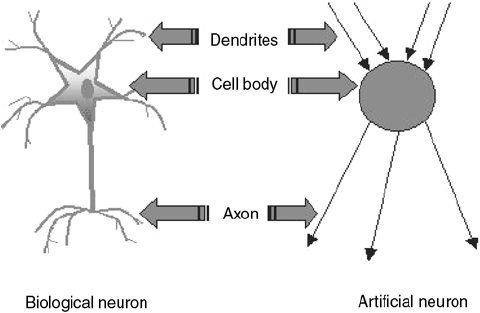
\includegraphics[height=4cm]{images/Fig-1-Analogy-between-artificial-neuron-and-biological-neuron.png}
	\caption{Biological and artificial neuron \cite{analogyneurons}}
	\label{fig:artifical_and_biological}
	\endminipage\hfill
	\minipage{0.4\textwidth}
	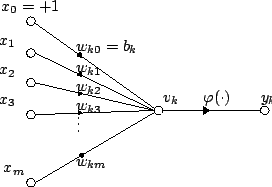
\includegraphics[height=4cm]{images/artificial_neuron.png}
	\caption{Single artificial neuron \cite{artificialneuron}}
	\label{fig:artificial_neuron}
	\endminipage
\end{figure}

\subsection{Neurons}
An artificial neuron is basically a mathematic function, aimed to imitate biological neurons.
As already mentioned, ANN have several things in common with biological neural networks, in this analogy, an artificial neuron is a simplified abstraction of a biological neuron, both have a cell body and incoming respectively outgoing connections, called dendrites and axons \cite{nntutorial} (Figure: \ref{fig:artifical_and_biological}). Every arriving signal over the dendrite is first multiplied with its corresponding weight, then added together. Be noted that $x_{0}$ is no input signal from a different neuron, but rather is a constant input of +1 and is called the bias input, it should get a mention, that the bias' weight is variable. \newline
After totalizing given input values, the signal is channeled through an activation function (also called transfer function) (Figure \ref{fig:artificial_neuron}). There are several possibilities for the transformation function to choose from. Its aim is to specify when the neuron produces actual output and when it remains silent. Another reason would be to keep the values between certain boundaries, usually, it is desirable to stay in ranges [0;1] or [-0.5;0.5], depending on the used transfer function. A Common transfer function would be the Sigmoid function (\ref{eqn:sigmoid}) although there are diverse other reasonable choices like the hyperbolic tangent function \cite{nntutorial}. Catching up with above-mentioned bias, it's purpose is to shift the activation function horizontally, the corresponding weight determines how much the function is being shifted(visualized in \ref{fig:sigmoid}). Coming back to previous analogy, the Sum-Operator in series connection with the Activation function form the artificial cell body.\newline 
After generating an output signal $y_{k}$ (\ref{eqn:dendrites_sum}), the Axon can fork into one or multiple branches, serving one or multiple neurons as it's or their input dendrites, needless to say,  after they have been weighted by their corresponding weights.   


\begin{equation}
\label{eqn:vk}
v_{k} = \sum_{i=0}^{m} x_{i} w_{ki}
\end{equation}  

\begin{equation}
\label{eqn:dendrites_sum}
y_{k} = \varphi(v_{k}) = \varphi(\sum_{i=0}^{m} x_{i} w_{ki}) 
\end{equation} 

\begin{equation}
\label{eqn:sigmoid}
S(x) = \frac{e^x}{e^x + 1} = \frac{1}{1 + e^{-x}}
\end{equation} 


\begin{figure}[H]
	\centering
	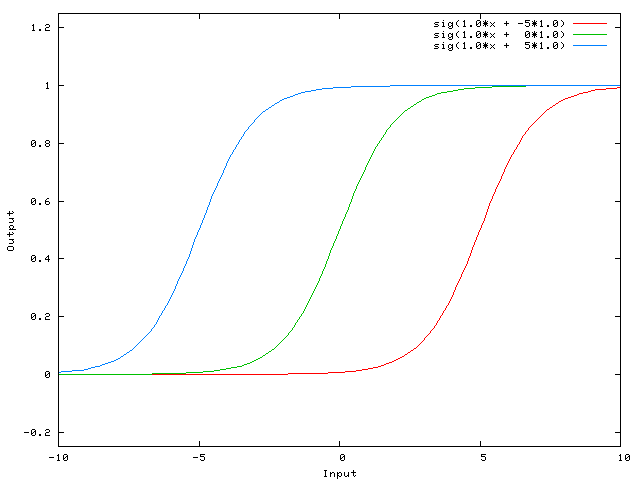
\includegraphics[width=\textwidth]{images/sigmoid.png}
	\caption{Sigmoid function with bias weight: 5 (blue), 0 (green), -5 (red){\cite{sigmoid}}}
	\label{fig:sigmoid}
	
\end{figure}


\subsection{From neurons To networks}
Feeding a signal or data through a neuron and transporting resulting output further to the next neuron(s) can be called a network. Now as the major purpose of artificial neural networks is to process any sort of data given to the ANN and produce some sort of output. Consequently, a model needs to have two different kinds of interfaces for importing and exporting data. \newline
The input part comprises a so-called input layer, containing several neurons that can be fed with data from outside of the network. Respectively there is the other end of the ANN, that produces a result after the calculation, performed by the net. Every neuron that is outputting data from the net is called output neuron, these neurons together form the output layer. The remaining neurons between input and output are named hidden neurons, they can be grouped in one or more hidden layers, depending on the defined architecture, normally each neuron of a layer $l_{n}$ has a connection to every neuron of its subsequent layer $l_{n+1}$.

\section{Common Types}
There are a lot of different types of neural networks, but digging deeper into the matter would definitely go beyond the scope of this discussion, so this section is going to be limited, to describe more or less shallowly only the two main types of ANNs \cite{nntutorial}. Regardless in which class a NN is categorized, as soon as it owns more than one hidden layer, the net can be classified as a deep neural network \cite{deep-learning-methods}. \newline
The type of architecture, which is being used in this project is called feedforward neural network (Figure: \ref{fig:ff_neural_net}), in this approach data, is only flowing in one direction, meaning from the Input Layer successively to the hidden layer(s) and at some point to the output layer, forming no cycles or loops. A before mentioned representative of this particular class is the convolutional neural network.\newline
In contrast to this, recurrent neural networks are slightly more complex than FFNN, because they add the directed cycles component, therefore these networks have internal memory to a certain extent, that is capable of forming dynamic temporal behaviour. 


\begin{figure}[H]
	
	\minipage{0.45\textwidth}
	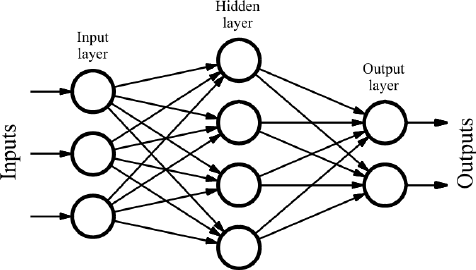
\includegraphics[height=3.5cm]{images/feed_forward_neural_net.png}
	\caption{Feed forward neural network \cite{ffnn}}
	\label{fig:ff_neural_net}
	\endminipage
	\hfill
	\minipage{0.5\textwidth}
	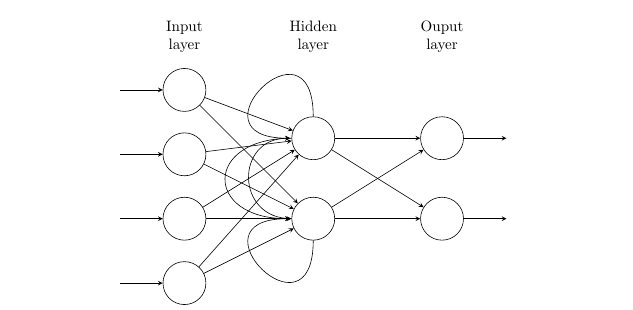
\includegraphics[height=3cm]{images/recurrent_neural_net.png}
	\caption{Recurrent neural network \cite{rnn}}
	\label{fig:rec_neural_net}
	\endminipage
\end{figure}

